\documentclass[letterpaper, 11pt]{article}

\usepackage{lastpage, marginnote, siunitx, circuitikz, kantlipsum, hyperref, amsmath}
\def\UrlBreaks{\do\/\do-}

%\usepackage[hyphens]{url}

\usepackage{geometry}
\geometry{hscale=.6, vscale=.8, hmarginratio=2:1, vmarginratio=1:1, marginparwidth=.18\paperwidth, ignoremp}
%\geometry{marginparwidth=.1\paperwidth}

%\usepackage[T1]{fontenc}

\usepackage[explicit]{titlesec}
\titlespacing*{\section}{\dimexpr -\marginparsep-\marginparwidth}{*4}{*1}
\titleformat{\section}[runin]{\large\bfseries\titlerule[.5pt]\filright}{\makebox[1em][c]{\thesection}}{1em}{\parbox[t]{\dimexpr\marginparwidth-0em}{#1}\hskip\marginparsep\mbox{}}[\newline\vspace{-0ex}]

%\titlespacing*{\subsection}{\dimexpr -\marginparsep-\marginparwidth}{*4}{*1}
%\titleformat{\subsection}[runin]{\large\bfseries\titlerule[.5pt]\filright}{\makebox[1em][c]{\thesection}}{1em}{\parbox[t]{\dimexpr\marginparwidth-2em}{#1}\hskip\marginparsep\mbox{}}[\newline]

\usepackage{enumitem}
\newlist{steps}{enumerate}{1}
\setlist[steps]{label=Step \arabic*, font=\bfseries, leftmargin=-\marginparsep, itemindent=\marginparsep, align=right}

\usepackage{fancyhdr}
\pagestyle{fancy}
\fancyhf{}
\fancyhfoffset[lh,lf]{\dimexpr\marginparwidth+\marginparsep}
\fancyhf[lh]{UCD EEC 134}
\fancyhf[ch]{}
\fancyhf[rh]{}
%\fancyhf[lf]{left foot}
%\fancyhf[cf]{centre foot}
\fancyhf[rf]{Page \thepage /\pageref{LastPage}}
%\renewcommand{\footrulewidth}{.4pt}

%%%%%%%%%%%%%%%
%%%% Tikz definitions
%%%%%%%%%%%%%%%
%\tikzstyle{Uno}=[rectangle,fill=white,draw,line width=0.5mm]

%new commands
%display due date in red and link to the eec134-schedule.pdf document
\newcommand{\due}[1]{\href{https://github.com/ucdart/UCD-EEC134/blob/master/support/schedule/eec134-schedule.pdf}{\textcolor{red}{#1}}}

\graphicspath{{./figures/}}

\begin{document}

\title{Lab 5: Antenna}
\author{Instructor: Xiaoguang ``Leo'' Liu\\lxgliu@ucdavis.edu \\
	\small \href{http://creativecommons.org/licenses/by-sa/4.0/}{CC BY-SA 4.0}}
\date{Last updated: \today}

\maketitle

In this project, we are going to use a coffee-can as the antenna. This may sound surprising at first but hopefully after you go through the above reference, it will become more apparent why it would work fairly well. The original idea of using a coffee can is attributed to Gregory Rehm\footnote{G. Rehm, ``How To Build A Tin Can Waveguide WiFi Antenna,'' [Online]. Available: \url{http://www.turnpoint.net/wireless/cantennahowto.html}. [Accessed 07 10 2013].}. 

	\begin{figure}[ht]
		\centering	
		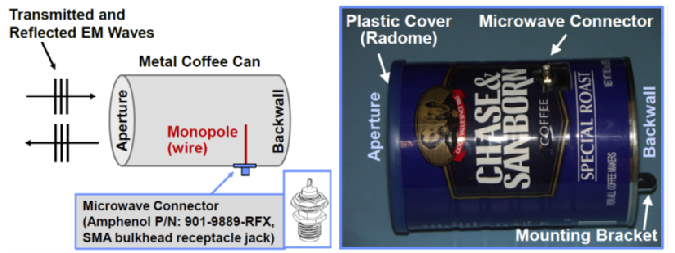
\includegraphics[width=4in]{coffee-can}
		\caption{Coffee can as an effective RF antenna.}
		\label{fig:coffee-can}
	\end{figure}
		
		
%\section{Objectives}
%
%\begin{enumerate}[itemsep=0.1ex]
%	\item Learn how to characterize RF mixers.	
%\end{enumerate}

%Be warned that this lab is a fairly aggressive one and it will take a lot of time for you and your group to finish all the reading, the pre-lab assignment, the actual lab, and the reports. It's a good idea to start early! And divide up tasks between group members wisely!

\section{Deliverables}
All items are to be submitted to the TA's email: eec134f2016@gmail.com.  

%\vspace{0.5cm}

\begin{table}[h]
	\footnotesize
	\caption{Lab 5 Deliverables}
	\renewcommand{\arraystretch}{1.2}
	\begin{tabular}{|m{1in}|l|m{0.45in}|m{2in}|}
		\hline
		\textbf{Item} & \textbf{Due date} & \textbf{Format} & \textbf{File name format} \\
		\hline
		\hline
		Pre-lab 5 & \due{Nov.~18th, 2018} & pdf & ``prelab-5-YourName.pdf''\\
				
		\hline
		Lab 5 report & \due{Nov.~25th, 2018} & pdf & ``lab-5-GroupName.pdf''\\
		\hline
	\end{tabular}
	\label{tab:deliverables}
\end{table}

\textbf{Notes:}
\begin{enumerate}
	\item All items are due by 11:59pm, of the due date. No late submissions are accepted. Don't even ask. 
	
	\item Please follow the file name format rigorously. Replace ``GroupName'' with your group's name and ``YourName'' with your name, first name first, last name last. 
\end{enumerate}


\section{Prelab}

The coffee-can is actually working as a cylindrical waveguide horn antenna. This means you cannot use any random coffee cans, it has to be quite conductive. To make sure that it is also mechanically reliable, we have picked ones made of aluminum. 

Similar to rectangular waveguides, cylindrical waveguides have many modes and each mode has a specific cut-off frequency. Typically, one would use the lowest order mode to prevent multiple mode propagation and conversion, which would cause signal degradation if not handled properly. 

The lowest order mode for a cylindrical antenna is the TE11 mode. Its cut-off wavelength is roughly 

\[
\lambda_c = 1.705 D,
\]
where $D$ is the diameter of the cylindrical antenna\footnote{N. Marcuvitz, Waveguide Handbook, Nework: MIT Radiation Laboratory Series, 1951}. Any frequency lower than $c/\lambda_c$ will not propagate inside the antenna, where $c$ is the speed of light. Therefore, the coffee can diameter needs to be large enough to make sure that it can work at the desired frequency ($\sim$2.4\,GHz in our case). 

For frequencies that are higher than the cut-off frequency, the guide wavelength $\lambda_g$, which is quite different from the free-space wavelength $\lambda$, is given by 
\[
	\lambda_g= \frac{\lambda}{\displaystyle \sqrt{1-\left( \frac{\lambda}{\displaystyle  1.705D} \right)^2}}.
\]

After making sure that the antenna can work at our desired frequency, we need to find a way to couple our signal into the antenna structure. One way to do this is to insert a short coaxial probe. The probe can be made from a coaxial line. The center conductor of the coaxial line extends into the antenna while the outer conductor is electrically connected to the antenna body. 

The hole needs to be $\lambda_g/4$ away from the bottom of the can. There is a simple explanation for this. Consider the probe feed to be an antenna itself (Fig.~\ref{fig:coffee-can-feed}). The radiated wave that propagates to the left will reflect on the bottom of the can with $\Gamma =-1$ (short circuit). In other words, the reflected wave experience a phase change of $\pi$. When the reflected wave arrives the feed probe again, it has experienced a total phase change of $\pi/2 + \pi + \pi/2 = 2 \pi$. This means that it is going to interfere constructively with the radiated wave propagating towards the right. Therefore radiation is enhanced with the probe being placed $\lambda_g/4$ from the bottom of the can. 

	\begin{figure}[ht]
		\centering	
		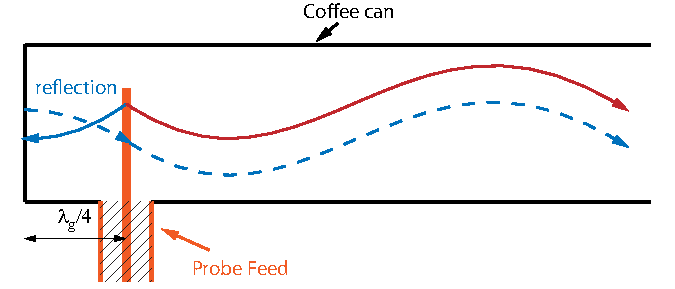
\includegraphics[width=4in]{coffee-can-feed}
		\caption{Feeding the coffee can antenna.}
		\label{fig:coffee-can-feed}
	\end{figure}

\reversemarginpar
\marginnote{\textbf{Pre-lab Assignment}\\\textbf{5}} 
\vspace{-2ex}
\begin{enumerate}
	\item Read the following materials and pay close attention to the concepts of antenna \textit{pattern}, \textit{main lobe}, \textit{side lobe}, \textit{half-power beam width (HPBW)}, \textit{radiation intensity}, \textit{directivity}, \textit{gain}, \textit{efficiency}, \textit{antenna aperture}, \textit{aperture efficiency}, \textit{polarization}, and the \textit{Friis formula}. 
	\begin{itemize}
		\item EEC 134 Lecture Note 7 
		
		\item John D.~Kraus and  Ronald J.~Marhefka, ``Antenna Basics,'' \emph{Antennas: For All Applications, 3rd Edition}, Chapter 2, 2001.
		
		\item John D.~Kraus and  Ronald J.~Marhefka, ``The Antenna Family,'' \emph{Antennas: For All Applications, 3rd Edition}, Chapter 3, 2001.
	\end{itemize}
	\item Read the Lab 5 procedures. 

	\item Please answer the following questions:
		\begin{enumerate}
			\item What is the difference between the \textit{directivity} and the \textit{gain} of an antenna? How are they related?
			
			\item What is the maximum power received at a distance of 0.5\,km over a free-space 1\,GHz circuit consisting of a transmitting antenna with a 25\,dBi gain and a receiving antenna with a 20\,dBi gain? The transmitting antenna input power is 150\,W. 
			
			\item What is the typical directivity of a half-wavelength dipole?
			
		\end{enumerate}

\end{enumerate}

\section{Equipment \& \\Supplies}

\begin{itemize}[itemsep=0.5ex]
	\item 1 $\times$ network analyzer (provided by the TA);
	\item 1 $\times$ GSP-730 spectrum analyzer;
	\item 2 $\times$ TPI synthesizer;
	\item 2 $\times$ 12'' and 2 $\times$ 6'' SMA cables;
	\item 2 $\times$ SMA female bulkhead adapter with receptor pin;
	\item 1 $\times$ electric drill tool and drill bits.
\end{itemize}


\section{Procedures}

\subsection{Antenna assembly and tuning}
\label{sec:antenna_assbly}

\begin{enumerate}
	\item Peel off the plastic wrapping on the coffee can. 

	\item Drill a hole in the coffee can using the Dremel tool provided by the TA. 
	\item Install the bulkhead SMA connector in the hole (Fig.~\ref{fig:drill}). Solder a piece of copper wire in the acceptor pin of the SMA connector. Make sure that the copper wire is longer than 2 inches so that you have enough room to cut it back.
	
		\begin{figure}[ht]
			\centering	
			\includegraphics[width=3.5in]{drill}
			\caption{The probe feed inside the coffee-can antenna.}
			\label{fig:drill}
		\end{figure}
	 
	
	\item With the help of the TA, measure the $S_{11}$ of the antenna using a vector network analyzer (VNA). When the antenna is radiating at the right frequency (2.4\,GHz in this lab), the $S_{11}$ should be at least better than -10\,dB. Your antenna may be initially off-resonance. Cut the copper in small increments until you get a good response on the VNA. Fig.~\ref{fig:s11} shows an example plot of a well-tuned antenna. 
		\begin{figure}[ht]
			\centering	
			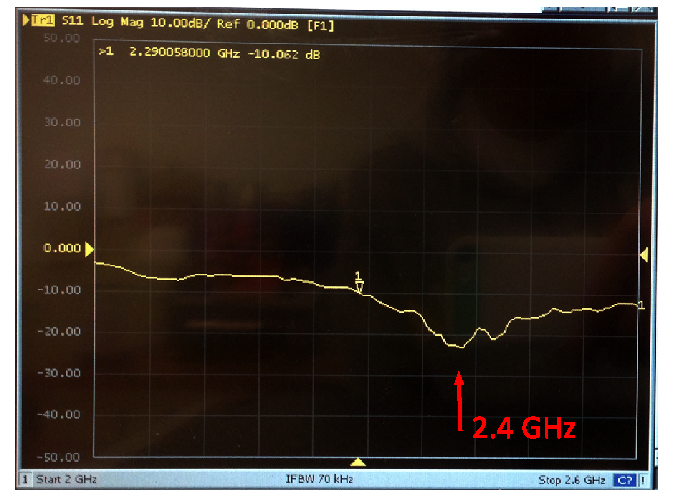
\includegraphics[width=3.5in]{s11}
			\caption{An example of a well tuned antenna's $S_{11}$.}
			\label{fig:s11}
		\end{figure}

	\item Repeat the above step for the second antenna. In your lab report, include pictures of your assembled antennas and plots of the measured $S_{11}$. What is the 10\,dB bandwidth of your antenna?  
		
\end{enumerate}

\subsection{Measuring Antenna Characteristics}

Antenna gain is generally measured using an anechoic chamber or antenna range. As a crude approximation of an antenna range, we could measure the gain of the antenna using the set-up in Fig.~\ref{fig:gain_measure}.
	\begin{figure}[ht]
		\centering	
		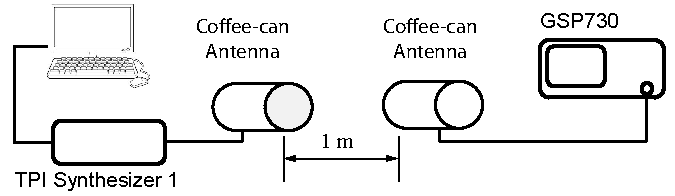
\includegraphics[width=4.5in]{gain_measure}
		\caption{Measuring antenna gain using two identical antennas.}
		\label{fig:gain_measure}
	\end{figure}
	
In this setup, two identical antennas are placed face to face with a distance of 1\,m apart. The received power on antenna 2 is roughly given by 
\[
	P_r = \frac{P_t}{\left( 4\pi r \right)^2} \lambda^2 G_1 G_2,
\]
where $P_t$ is the transmitted power from antenna 1, $r = 1$\,m, $G_1$ and $G_2$ are the gains of the antennas. Since the two antennas are essentially identical, $G_1 = G_1$. Therefore, the gain of the antenna can be expressed by 
\begin{equation}
	G = G_1 = G_2 =\frac{4\pi r}{\lambda}\sqrt{\frac{P_r}{P_t}}.
	\label{eqn:gain}
\end{equation}

\begin{enumerate}
	\item Connect the TPI synthesizer to one of your antennas. Set the output frequency and power of the synthesizer to 2.4\,GHz and 0,dBm (this will be your $P_t$)
		
	\item Connect the other antenna to the GSP-730 spectrum analyzer. 
	
	\item Place the antennas 1\,m apart, facing each other. Make sure that the feed pins of the two antennas are aligned in the same direction. 
	
	\item \textbf{Antenna Gain}	You should be able to measure a signal at 2.4 GHz on your spectrum analyzer. Record the power of this signal, which will be your $P_r$) and calculate the gain of your antennas using \eqref{eqn:gain}. Make sure that you carefully take into account the loss of the connectors, adapters, and cables. 
	
	\item \textbf{Cross-polarization} Now rotate one of the antennas 90$^\circ$ axially so that the two feed pins are perpendicular to each other  (the antennas should still face each other). Record the power of the received signal. Explain the difference in the received powers in Step 4 and 5. 
	
	\item \textbf{(Optional) Antenna Pattern } After you have finished the above steps, the TA can show you to the anechoic chamber in the Kemper 3182 lab, where you can have the pattern of your antenna measured. Plot the pattern of your antenna in your lab report. Alternatively, you may also try to do a crude pattern measurement by yourself. Fig.~\ref{fig:pattern_measure} will give you some hint. Ask the TA for the reference 2.4\,GHz antenna. 
		\begin{figure}[ht]
			\centering	
			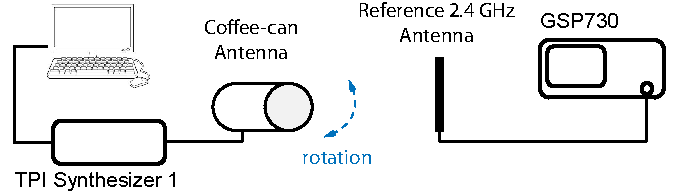
\includegraphics[width=4.5in]{pattern_measure}
			\caption{Measuring antenna pattern using a reference antenna.}
			\label{fig:pattern_measure}
		\end{figure}
\end{enumerate}
%\newpage
%\begin{thebibliography}{9}
%
% 
%\bibitem{thomas-sa}
%Jeff Thomas, Tom Holmes, Terri Hightower, ``Learn RF Spectrum Analysis Basics,'' Agilent Technologies, \url{https://www.jlab.org/uspas11/Reading/RF/RF%20Spectrum%20Analysis.pdf}.
%
%\bibitem{diez-sa}
%Erik Diez, ``The Fundamentals of Spectrum Analysis,'' Agilent Technologies, \url{http://electronicdesign.com/test-amp-measurement/fundamentals-spectrum-analysis}.
%
%
%\end{thebibliography}

\end{document}